% !TeX encoding = UTF-8
% !TeX program = pdflatex

\documentclass[11pt]{article}
\usepackage{graphicx}

\title{{\bf The usage and the impact of shift registers on the CFB mode of operation} \\ \bigskip \large HW1 - CNS Sapienza}
\date{2018-10-12}
\author{Andrea Fioraldi 1692419}
\pagenumbering{roman}

\begin{document}
\maketitle

\section{Introduction}

With the aim to provide confidentiality and authenticity of information, {\em Block Ciphers} are widely used in cryptography. Block Chiphers operates on fixed-length messages, called {\em blocks}, and {\em Modes of Operations} are the techniques used to apply block chiphers to messages longer than a block.

{\em Cipher Feedback} (CFB) is a popular mode of operation. In this technique, regards the ecryption, the produced cyphertext block xored with the corrispindendt plaintext block is forwarded to the next encryption unit to produce the next cyphertext block. 

\begin{figure}[!ht]
  \centering
  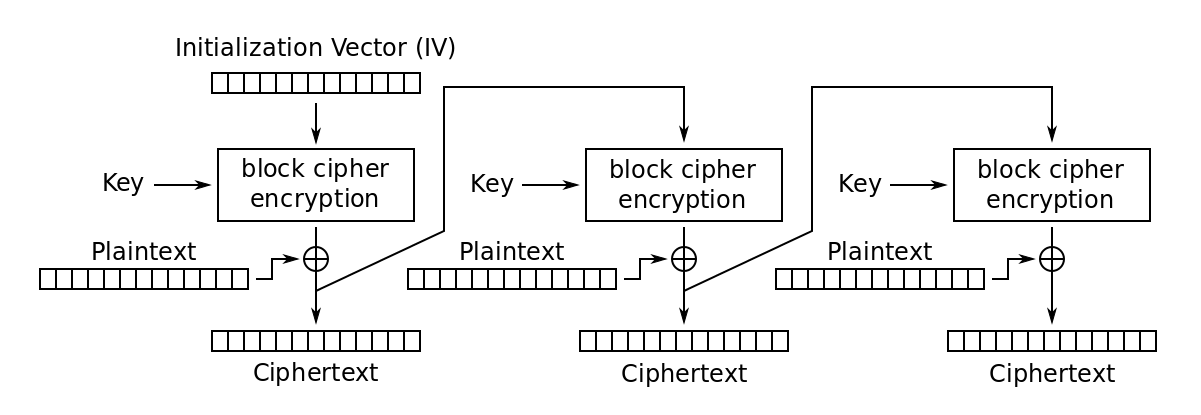
\includegraphics[width=1\textwidth]{pic1-hw1-1692419}
  \caption{CFB encryption, from \cite{wiki}}
  \label{fig:cfb_enc}
\end{figure}

Viceversa, during the decryption, the produced plaintext xored with the correspondent cyphertext is forwarded to produce the next plaintext block.

\begin{figure}[!ht]
  \centering
  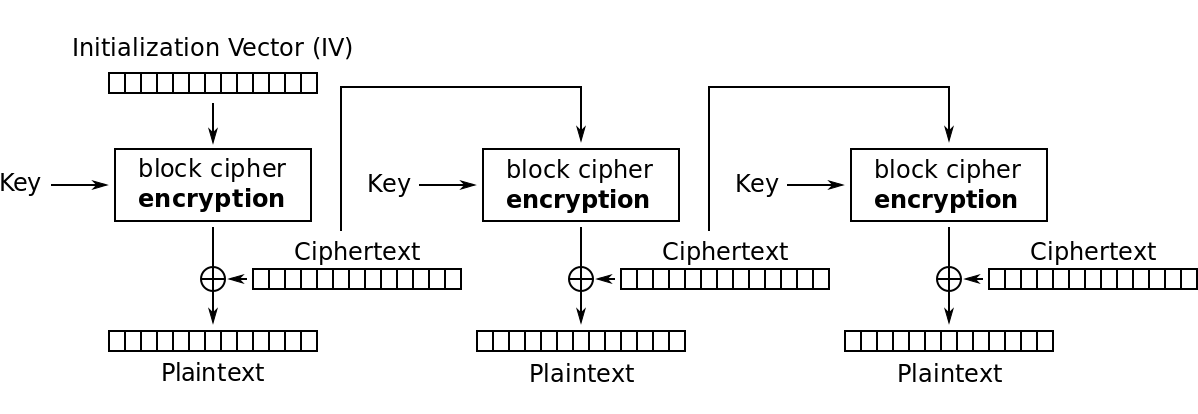
\includegraphics[width=1\textwidth]{pic2-hw1-1692419}
  \caption{CFB decryption, from \cite{wiki}}
  \label{fig:cfb_dec}
\end{figure}

This mode of operation requires an initialization vector (IV) as initial input block. As you can see in figure \ref{fig:cfb_dec} the encryption unit is used also for decryption.

\section{Shift registers}

One of the most used variant of CFB introduces shift registers as input for the encryption unit.

\subsection{Usage}



\begin{figure}[!ht]
  \centering
  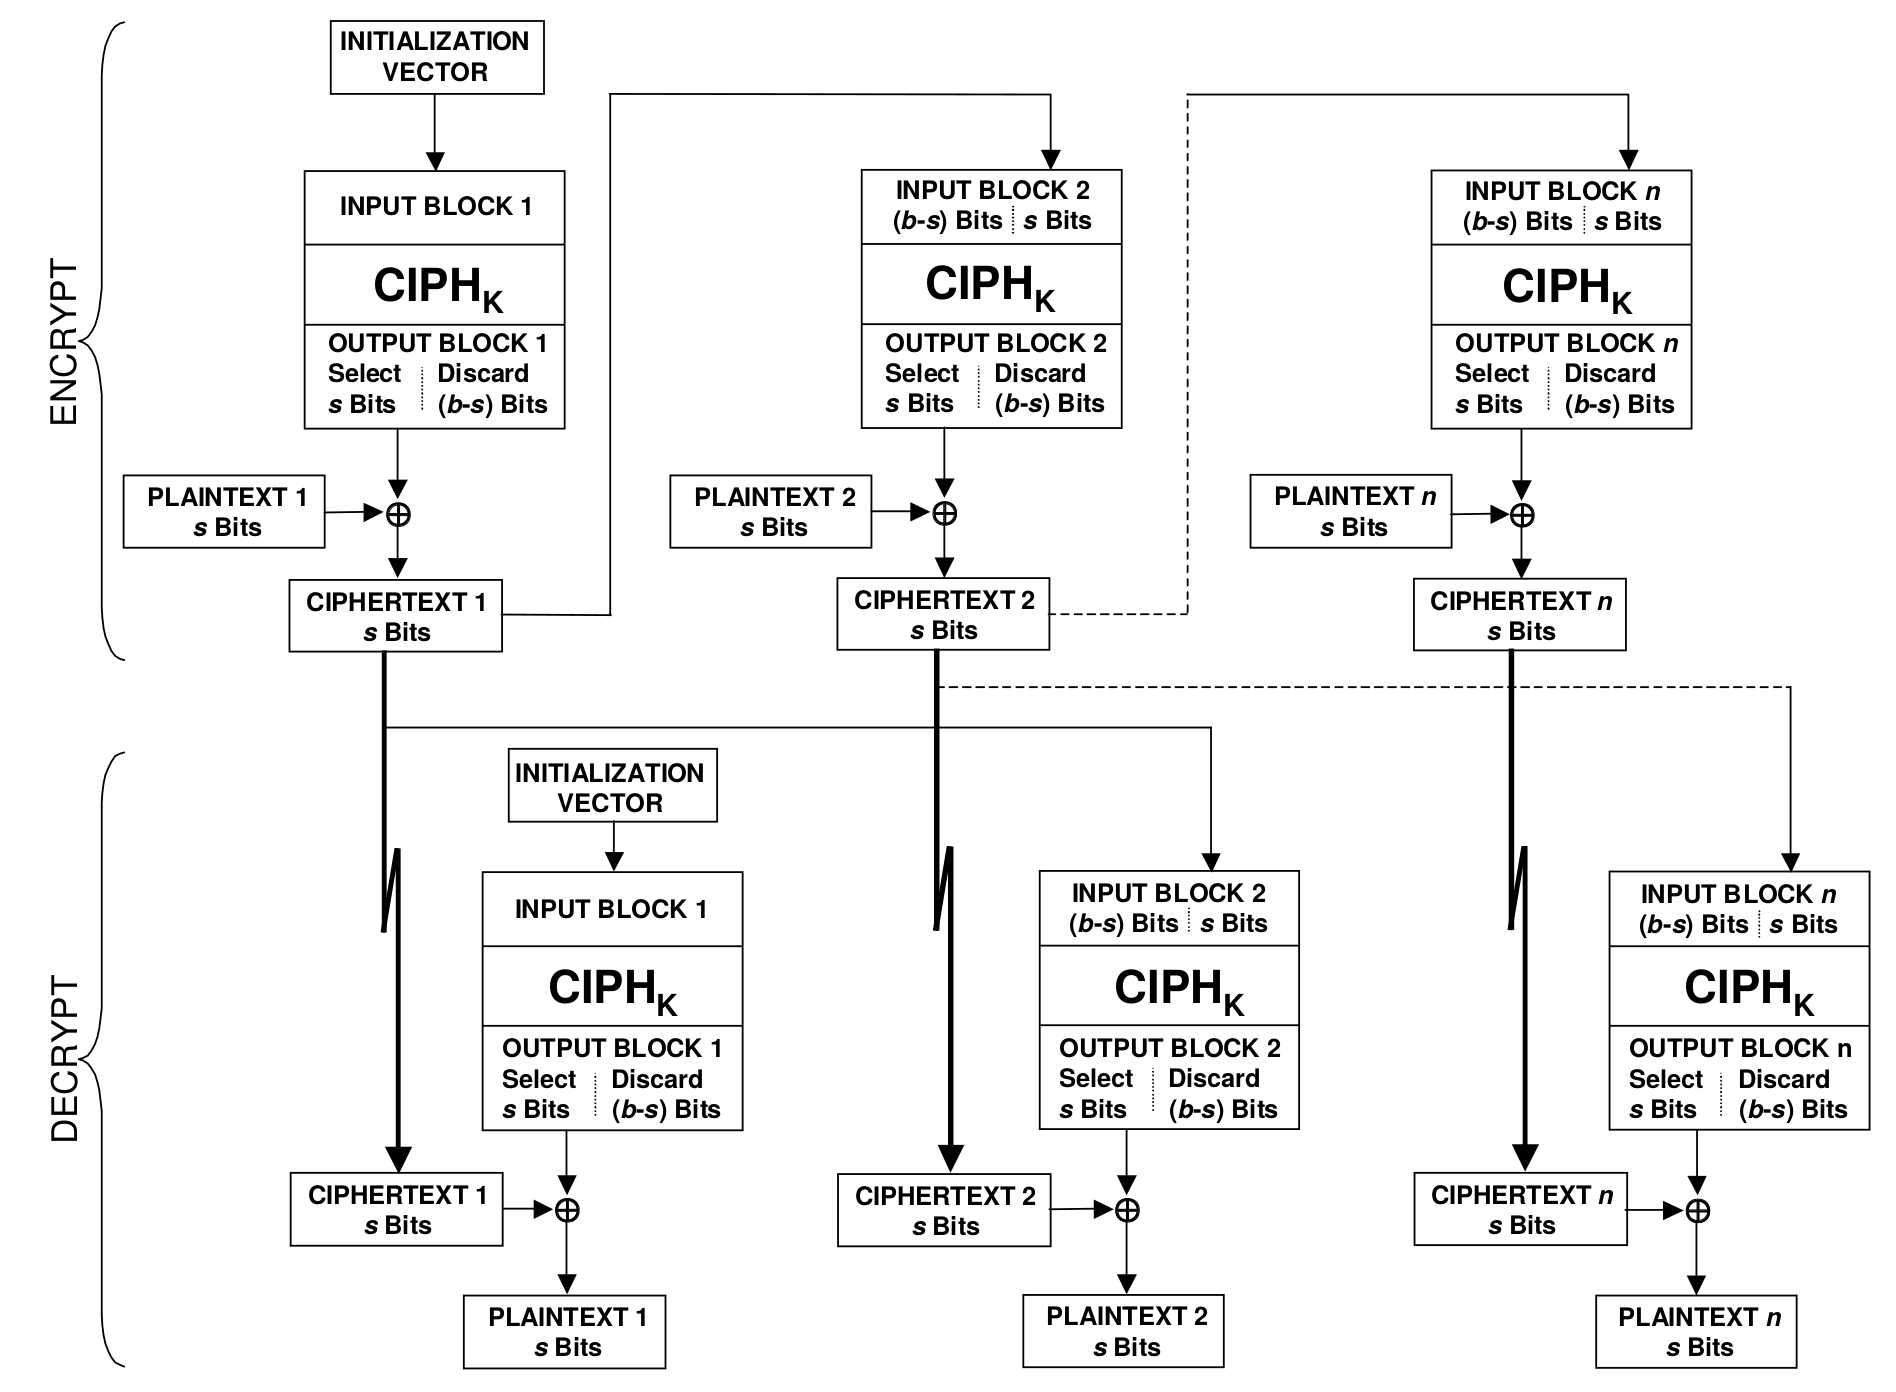
\includegraphics[width=1\textwidth]{pic3-hw1-1692419}
  \caption{CFB with shift registers, from \cite{nist}}
  \label{fig:cfb_shift}
\end{figure}

\subsection{Impact}



\newpage
\begin{thebibliography}{10}

\bibitem{wiki}
{\em Block cipher mode of operation - Wikipedia}.
  \verb|https://en.wikipedia.org/wiki/Block_cipher_mode_of_operation|.
  \newblock Accessed: 2018-10-12.

\bibitem{nist}
Morris Dworkin.
  {\em Recommendation for Block Cipher Modes of Operation. Methods and Techniques}.
  Tech. rep. 800-38A. National Institute of Standards and Technology, 2001.
  \newblock \verb|url: http://www.dtic.mil/docs/citations/ADA400014|.

\end{thebibliography}

\end{document}
